\documentclass[compress]{beamer}
\usepackage[
    title={UFFA Points System},
    subtitle={Un sistema a punti per la distribuzione equa dei turni di lavoro},
    event={UFFA Points System},
    author={Daniele La Prova},
    longauthor={Daniele La Prova 0320429},
    email={daniele.laprova@students.uniroma2.eu},
    institute={CSW 2022-2023},
    longinstitute={Universita' degli Studi di Roma Tor Vergata},
]{unislides}

\begin{document}
    
\begin{frame}[plain]
    \titlepage
\end{frame}

\section{Scenario}
\begin{frame}{\secname}
    \onslide<+-> \begin{itemize}
        \item Il problema consiste nell'escogitare un algoritmo capace di assegnare
        i turni di lavoro tra i membri del personale medico;
        \item La distribuzione deve avvenire nella maniera più equa possibile, ovvero
        rispettando le preferenze dei lavoratori e cercando di evitare che sempre le
        stesse persone debbano lavorare in giorni festivi o in turni scomodi;
    \end{itemize}
    \onslide<+-> \begin{alertblock}{}
        \textbf{È importante che il personale minimo necessario a
        svolgere un turno sia sempre reperito} , ovvero questo vincolo deve
        prevalere su qualunque altro.        
    \end{alertblock}
\end{frame}
\begin{frame}{\secname}
    \onslide <+-> \begin{itemize}
        \item Si supponga che il sistema disponga di un insieme di \texttt{Turni}:
        \begin{itemize}
            \item Ogni Turno porta con sé un insieme di attributi;
            \item È necessario che ad ogni Turno vengano allocati uno o più impiegati
            per svolgerlo.
        \end{itemize}
    \end{itemize}
    \onslide<+-> \begin{block}{\textbf{Idea}}
        Per ogni turno, il sistema seleziona un impiegato e ipotizza la sua allocazione
        per quel turno, dunque calcola quanti UFFAs questa allocazione ha generato.
        Il candidato effettivamente allocato sarà quello che minimizza il punteggio
        UFFA che ne consegue.
    \end{block}
\end{frame}

\section{Calcolo UFFA points}
\subsection{Scocciature}

\begin{frame}{\subsecname}
    \begin{itemize}
        \item Per ogni dipendente esistono delle \texttt{Scocciature};
        \item Una Scocciatura descrive un insieme di vincoli applicati sugli attributi
        di un Impiegato e del Turno a cui deve essere allocato;
        \item Ogni vincolo descrive anche un punteggio UFFA che rappresenta il valore
        della sua infrazione;
        \item La somma degli UFFA dei vincoli violati di una Scocciatura ne determina il
        suo puntegggio, e la somma dei punteggi delle Scocciature di un Turno ne
        determina il suo punteggio UFFA complessivo.
    \end{itemize}
\end{frame}
\begin{frame}{\subsecname}
    \begin{figure}
        \centering
        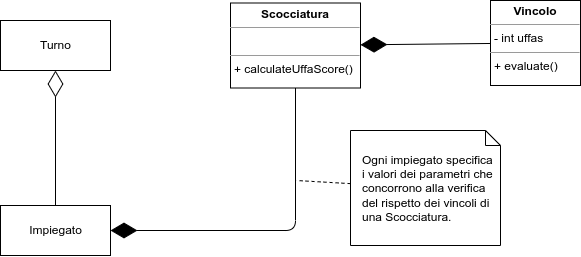
\includegraphics[width=\textwidth]{./figs/examples.png}
        \caption{Diagramma che descrive la relazione tra le entità del sistema}      
    \end{figure}
\end{frame}

\section{Esempi}
\begin{frame}{\secname}
    \begin{exampleblock}{Impiegato in Malattia}
        Tale Scocciatura presenta come vincolo quello di non assegnare un turno i cui
        giorni si sovrappongano a quelli di malattia dell'impiegato. L'infrazione di
        tale vincolo comporta un esorbitante quantitativo di UFFA, rendendo
        l'allocazione di questo impiegato a questo turno possibile solo se davvero non
        si trova di meglio.
    \end{exampleblock}
\end{frame}
\begin{frame}{\secname}
    \begin{exampleblock}{Natale al lavoro}
        Un impiegato che ha espresso la preferenza di non lavorare in giorni festivi
        può essere modellato con una Scocciatura con un vincolo il cui punteggio UFFA
        sia proporzionale al numero di giorni festivi consecutivi passati al lavoro.
    \end{exampleblock}    
\end{frame}

\section{Conclusioni}
\subsection{Vantaggi}
\begin{frame}{\subsecname}
    \begin{itemize}
        \item Non esistono situazioni in cui non è possibile trovare un candidato
        ammissibile per l'allocazione di un turno. Ciò è molto importante per un luogo
        come l'ospedale, che non può mai chiudere.
        \begin{itemize}
            \item Al limite, si troverà un candidato la cui assegnazione al turno
            genera un punteggio UFFA molto alto. Vorrà dire che passerà molto tempo
            prima che venga scelto nuovamente per turni che vanno contro le sue
            preferenze;
        \end{itemize}
        \item Dividere una Scocciatura in più vincoli ne facilita l'aggiornabilità,
        poiché così è possibile implementare varianti attenuate della stessa
        Scocciatura semplicemente scomponendone la logica in più vincoli;
        \begin{itemize}
            \item Più vincoli sono violati, più il punteggio UFFA sarà vicino al valore
            pieno;
        \end{itemize}
        \item Trovare un candidato ottimo per un turno ha costo pari a $N$ impiegati
        per $S$ scocciature per $V_s$ vincoli di ogni scocciatura. Tuttavia, non è
        necessario ricorrere alla PL.
    \end{itemize}
\end{frame}
\subsection{Problemi}
\begin{frame}{\subsecname}
    \begin{itemize}
        \item Come parametrizzare vincoli?
        \item Come assegnare gli UFFAs per ogni vincolo?
        \item È abbastanza veloce?
        \item ???
    \end{itemize}
\end{frame}

\end{document}